\documentclass{article}
\title{Janim Example 1}
\author{John Doe}
\usepackage{tikz}
\usepackage{geometry}
\geometry{
paperheight=216mm,paperwidth=384mm,
total={344mm,176mm},
left=20mm,
top=20mm,
}
\usepackage{fontspec}
\usepackage{xcolor}
\setmainfont{CascadiaMono.ttf}
\pagenumbering{gobble}
\pagecolor{black}
\hyphenpenalty 10000
\exhyphenpenalty 10000
\begin{document}
\maketitle
\noindent \textcolor{white}
{\Huge \textcolor{cyan}{Basic Shapes}}
\noindent \textcolor{white}
{\vspace{5mm}}
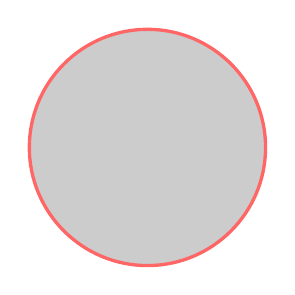
\begin{tikzpicture}
\filldraw[color=red!60, fill=black!20, very thick](20mm,40mm) circle (15mm);
\end{tikzpicture}
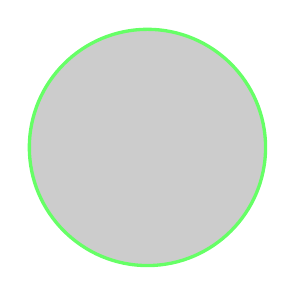
\begin{tikzpicture}
\filldraw[color=green!60, fill=black!20, very thick](60mm,40mm) circle (15mm);
\end{tikzpicture}
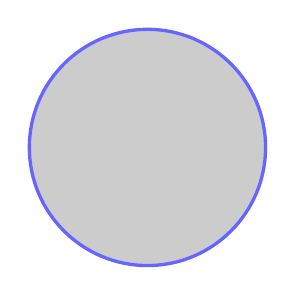
\begin{tikzpicture}
\filldraw[color=blue!60, fill=black!20, very thick](100mm,40mm) circle (15mm);
\end{tikzpicture}

\begin{tikzpicture}
\filldraw[color=magenta!60, fill=black!20, very thick](20mm,80mm) rectangle (20mm+20mm,80mm+20mm);
\end{tikzpicture}

\begin{tikzpicture}
\filldraw[color=yellow!60, fill=black!20, very thick](60mm,80mm) rectangle (60mm+20mm,80mm+20mm);
\end{tikzpicture}

\begin{tikzpicture}
\filldraw[color=cyan!60, fill=black!20, very thick](100mm,80mm) rectangle (100mm+20mm,80mm+20mm);
\end{tikzpicture}

\begin{tikzpicture}
\filldraw[color=orange!60, fill=black!20, very thick](30mm,120mm) -- (30mm+20mm,120mm) -- (30mm+20mm/2,120mm+20mm) -- cycle;
\end{tikzpicture}
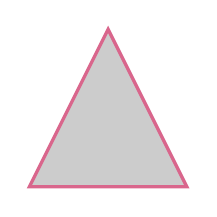
\begin{tikzpicture}
\filldraw[color=purple!60, fill=black!20, very thick](70mm,120mm) -- (70mm+20mm,120mm) -- (70mm+20mm/2,120mm+20mm) -- cycle;
\end{tikzpicture}
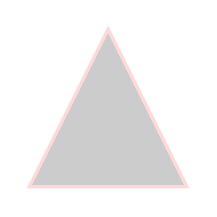
\begin{tikzpicture}
\filldraw[color=pink!60, fill=black!20, very thick](110mm,120mm) -- (110mm+20mm,120mm) -- (110mm+20mm/2,120mm+20mm) -- cycle;
\end{tikzpicture}
\begin{tikzpicture}
\draw[color=white, thick] (35mm,55mm)--(45mm,70mm);
\end{tikzpicture}
\begin{tikzpicture}
\draw[color=white, thick] (75mm,55mm)--(85mm,70mm);
\end{tikzpicture}
\begin{tikzpicture}
\draw[color=white, thick] (115mm,55mm)--(125mm,70mm);
\end{tikzpicture}
\noindent \textcolor{white}
{\vspace{20mm}}
\noindent \textcolor{white}
{\textcolor{white}{This document demonstrates basic geometric shapes in Janim:}}
\noindent \textcolor{white}
{\begin{itemize}}
\noindent \textcolor{white}
{\item \textcolor{red}{Red}, \textcolor{green}{green}, and \textcolor{blue}{blue} circles}
\noindent \textcolor{white}
{\item \textcolor{magenta}{Magenta}, \textcolor{yellow}{yellow}, and \textcolor{cyan}{cyan} squares}
\noindent \textcolor{white}
{\item \textcolor{orange}{Orange}, \textcolor{purple}{purple}, and \textcolor{pink}{pink} triangles}
\noindent \textcolor{white}
{\end{itemize}}
\end{document}
